\chapter{引言}\label{chap:Introduction}
%%%%%%%%%%%%%%%%%%%%%%%%%%%%%%%%%%%%%%%%%%%%%%%%%%%%%%%%%%%%%%%%%%%%%%
\section{研究背景与意义}\label{sec:background_and_motivation}
    \subsection{存算性能剪刀差与存储墙}\label{subsec:memory_wall}

    随着科技和信息化进程的持续加速,计算技术已经成为支持现代社会发展的关键基石。为了满足不断增长的高性能计算需求以及层出不穷的新型负载,计算机系统结构研究者正面临着一系列挑战。  
    
    在过去的几十年中,受益于集成电路制造工艺和封装技术的飞速演进,通用处理器技术的迭代一直是推动高性能计算系统计算能力增长的中坚力量。然而在如今,尤其是在面对新型高性能计算负载时,如生物信息学、数据库和图计算负载时,主存储器和CPU核心之间的数据搬移在
    延迟\citep{hashemi_accelerating_nodate}和能耗\citep{pandiyan_quantifying_2014}方面都产生了不可忽视的开销,通用处理器正逐渐显露出其架构与生俱来的局限性。此外,如图~\ref{fig:hw_scaling}所示,处理器与存储器在发展中性能所形成的“剪刀差”,加剧了计算过程中由数据搬移所形成的访存瓶颈,构成了通用计算系统能耗的显著比重\citep{denning_exponential_2016}。该现象早在上世纪末就被研究者广泛地意识到,此后被相关领域研究者统称为存储墙(Memory Wall)\citep{wulf_hitting_1995}问题。而随着此前通用处理器发展所遵循的摩尔定律\citep{moore_cramming_1998}和丹纳德缩放定律\citep{dennard_design_nodate}在二十世纪初的先后放缓或失效,处理器的功耗随其运行频率的增长而急剧增加,这也限制了单一处理器计算密度和规模的进一步提升。对冯诺依曼体系结构下的新型计算机系统结构、乃至非冯诺依曼体系结构的设计,已经成为诸多高性能计算系统工作的焦点。
    
    \begin{figure}[!htbp]
        \centering
        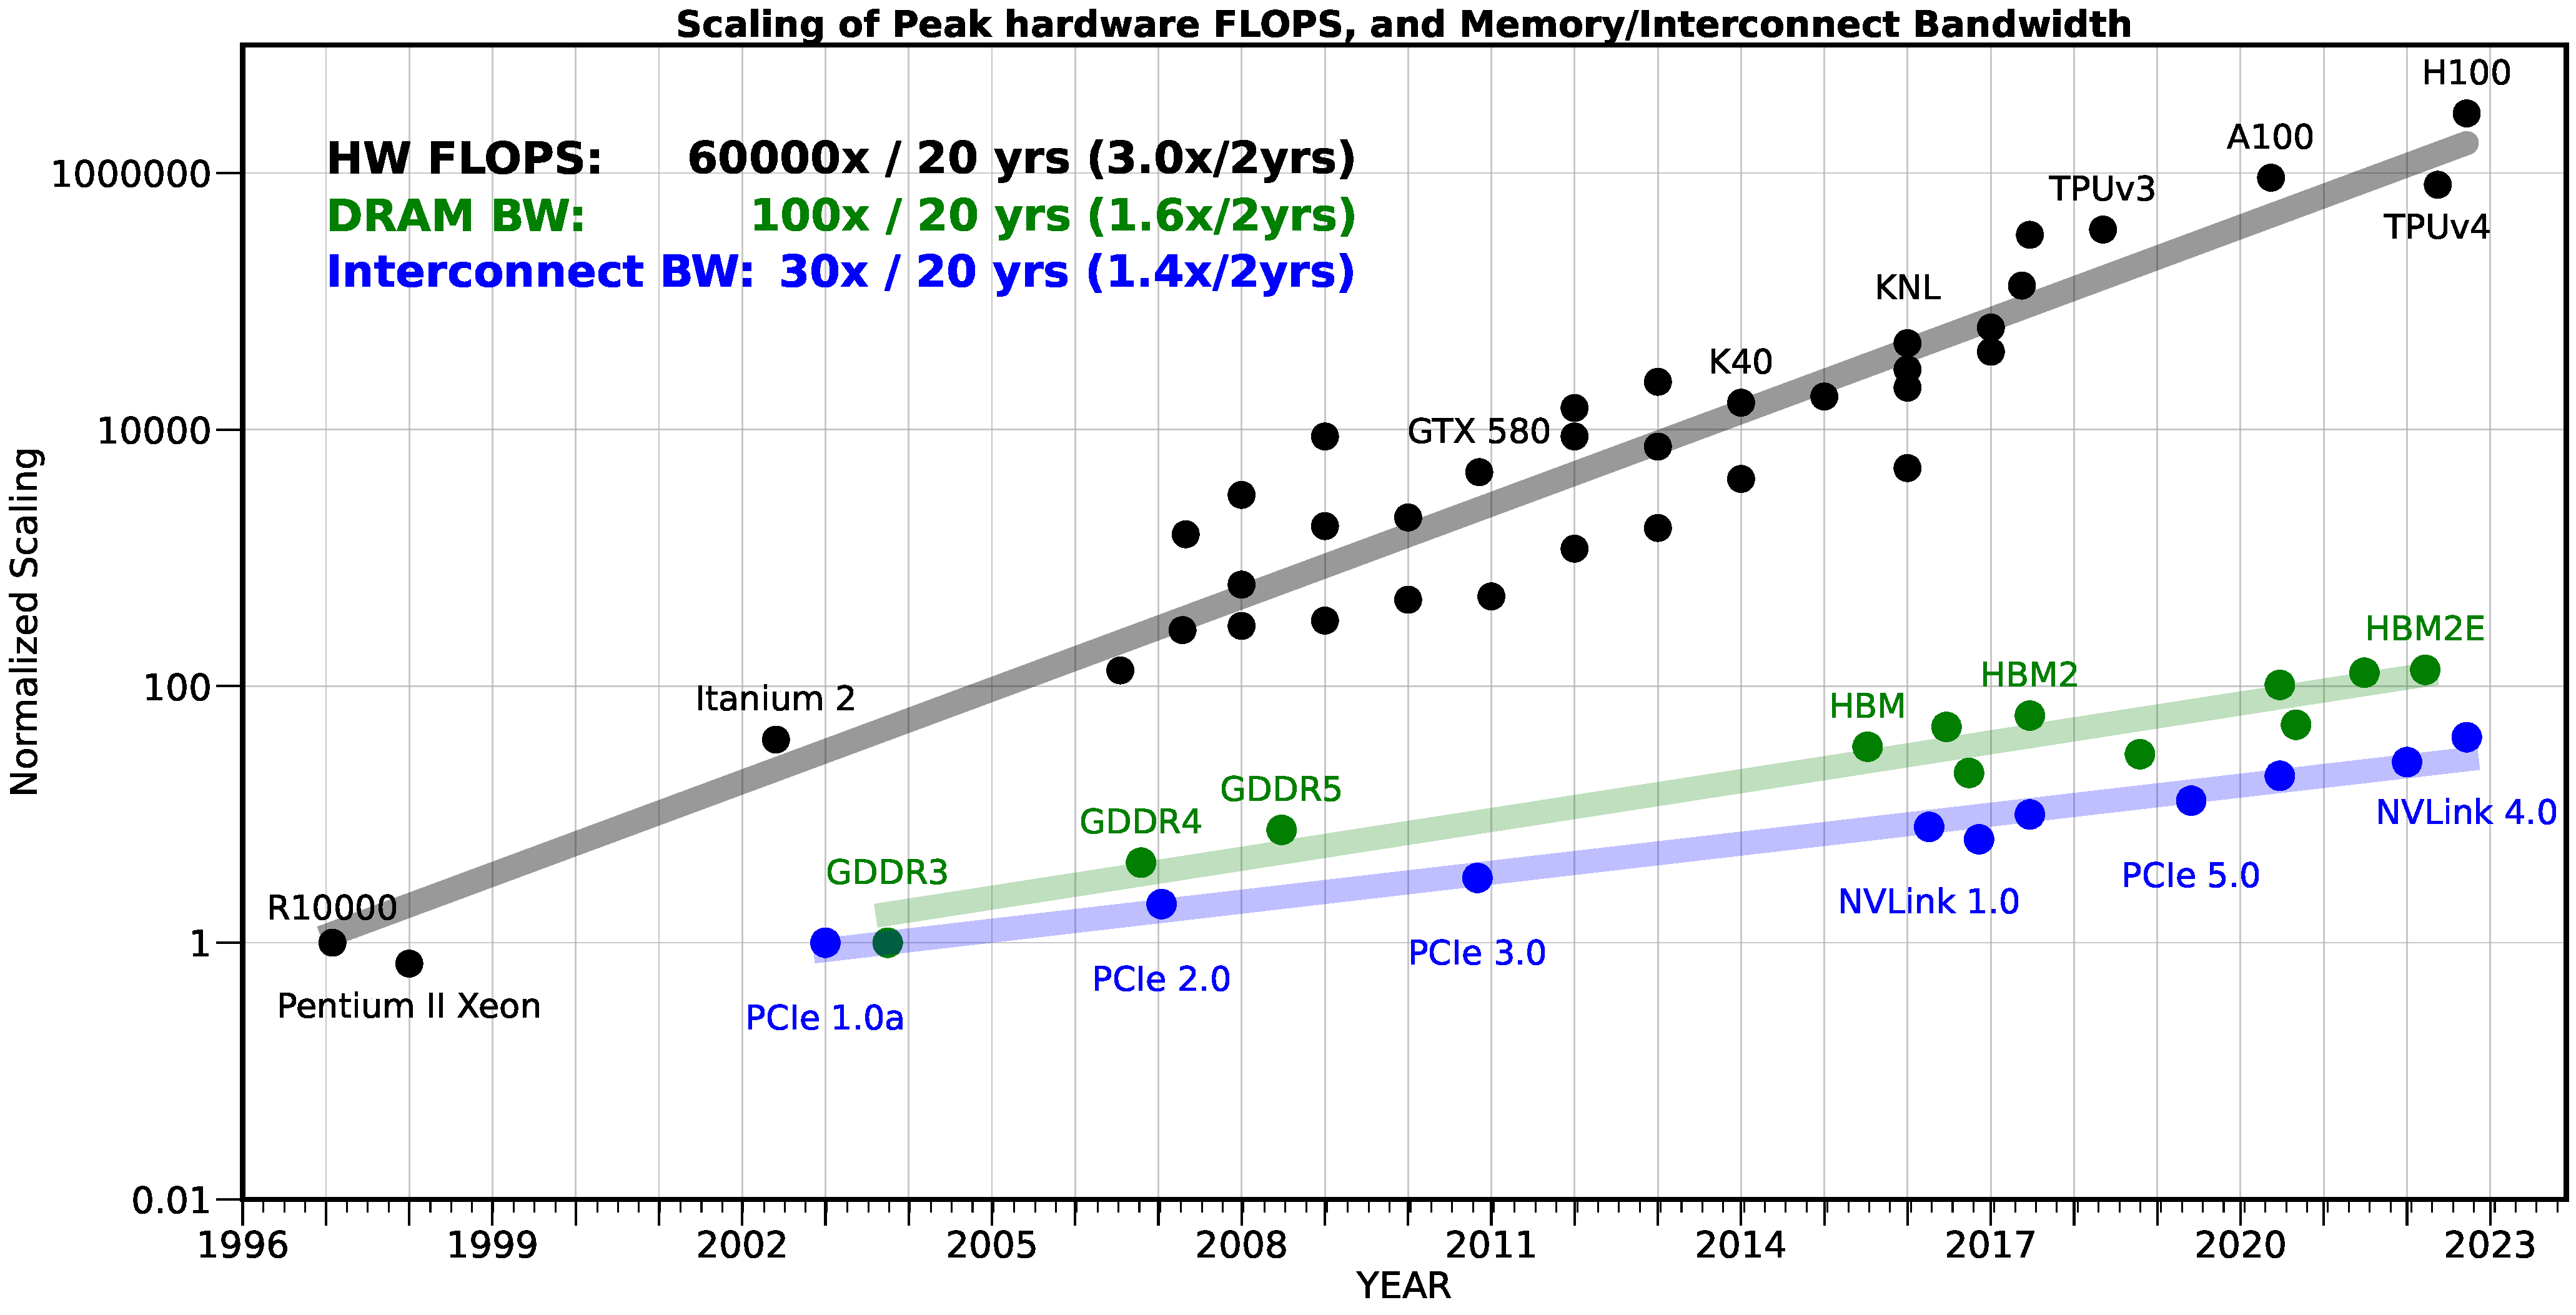
\includegraphics[width=0.85\textwidth]{hw_scaling}
        \bicaption{\quad 计算-存储-互联性能剪刀差示意图\citep{gholami_ai_2023}}
        {\quad Illustration of Compute-DRAM-Interconnect performance gap\citep{gholami_ai_2023}}
        \label{fig:hw_scaling}
    \end{figure}
    
    在高性能计算领域,许多工作负载之所以面临“存储墙”问题,根本原因在于处理器在执行某些计算密集型任务时,必须频繁地通过高延迟、低带宽的内存总线进行数据搬移。这些任务往往具有较差的时间-空间局部性,其中的数据复用不足以抵消或分摊主存储器访问的时间成本。随着存储和计算单元在延迟和带宽上的差距日益扩大,数据搬移导致的性能瓶颈在高性能计算任务中变得日益显著。

    在稀疏矩阵计算中,矩阵数据展现的不同稀疏模式以及采用的矩阵压缩方式对算法性能都有着显著的影响。这类算法普遍具有大量随机访存特性,因此其性能在很大程度上受到访存性能的限制。
    
    在生物信息学领域,基因序列比对和变异分析是关键的计算负载。当前被广泛使用的二代基因测序技术能够在一次全基因测序中产生总量高达数十甚至数百GB的基因读序,这些读序长度通常为数百个字符。在考虑多种变异的情况下,将这些读序精确地比对到共有数十亿碱基对的人类基因组中,是对存储系统性能的严峻挑战。序列比对过程中几乎不涉及密集的浮点运算和整数乘除法,而是涉及大量位运算和整数加减法,伴随着大跨度、随机性强、局部性差的访存模式。

    在数据库领域,关系型数据库中的join操作是一种出现频率高且十分耗时的操作。由于涉及多个表的数据操作、复杂的连接条件以及数据分布的不均匀性,尽管这类操作易于书写和理解,其性能问题却一直广受诟病。因此,对这类操作的规避和等价替换成为提升数据库性能的常见策略。
    
    \subsection{近存计算技术的发展}\label{subsec:evolution_of_PNM}
    为了从根本上缓解数据搬移开销所带来的访存瓶颈,另一种计算范式走上了历史舞台,这种范式通过把计算能力“下放”给主存储器模块,从而使其在计算中发挥主动作用。
    
    在狭义上,区别于是否真正对内存的硬件结构做出修改,该范式中的一部分实现被称为“近存计算”(Processing-Near-Memory,PNM),但其通常也与另一类实现——“可计算存储”(Processing-Using-Memory, PUM)被统称为广义上的“存内计算”(Processing-In-Memory, PIM):前者在存储单元附近集成计算逻辑,如\citep{chang_energy-efficient_2021}\citep{fernandez_natsa_2020}后者直接改变存储单元物理结构以使得其拥有计算能力,如\citep{tu_multcim_2023}\citep{zhang_edge_2023},区别于设计理念与具体的技术实现,广义的存内计算概念可以按表~\ref{tab:PIM-category}分为若干类别

    \begin{table}[!htbp]
        \bicaption{\quad 存内计算范式的设计理念与技术实现}{\quad PIM Approaches and Technologies}
        \label{tab:PIM-category}
        \centering
        \footnotesize% fontsize
        \setlength{\tabcolsep}{4pt}% column separation
        \renewcommand{\arraystretch}{1.2}%row space 
        \begin{tabular}{cl}
            \hline
            设计理念 & 技术实现\\
            %\cline{2-9}% partial hline from column i to column j
            \hline
            可计算存储 (PUM)&\begin{tabular}{l}
                                    基于SRAM\\
                                    基于DRAM\\
                                    基于相变内存(Phase-change memory, PCM)\\
                                    基于磁记忆体(Magnetic RAM, MRAM)\\
                                    基于忆阻器(Resistive RAM, RRAM)
                                    \end{tabular}\\
            \hline
            近存计算 (PNM)&\begin{tabular}{l}
                                    基于3D堆叠内存中的逻辑层\\
                                    基于硅中介层(Silicon interposers)附加逻辑\\
                                    基于近内存控制器附加逻辑\\
                                    基于近内存颗粒附加逻辑\\
                                    基于近内存模块附加逻辑\\
                                    基于近缓存附加逻辑\\
                                    基于近储存设备附加逻辑
                                    \end{tabular}\\
            \hline
        \end{tabular}
    \end{table}
    
    其中,近存计算技术的核心思想是将通过向存储单元附近集成计算元件,将计算能力下放到内存系统中,以减少数据在主存储器和CPU之间的频繁移动,从而在访存密集型工作负载运行时降低延迟和能源消耗\citep{mutlu_modern_2022}。而本课题所涉及到的基于DIMM的近存计算技术则是对现有的DIMM内存模块进行定制,将计算能力集成在内存颗粒之中,从而实现近存计算。通过将计算与内存紧密结合,PIM技术有望从根本上均摊计算访存强度不匹配时数据移动的开销,从而改善内存密集型工作负载的性能。
    
    由于以UPMEM为主的众多近存计算系统在相当多的文献中将自己所属的范式归类为“存内计算(PIM)”,本文为了在简洁的同时避免“大端小端”式的混淆,后续所提到的“PIM”及“存内计算”,若未特别指出,均指的是Processing-Near-Memory, 即特指“近存计算”。
    
    \subsection{近存计算技术所面临的挑战}\label{subsec:challenge_for_PNM}
    近存计算系统作为一种特殊的系统结构,在面对访存瓶颈负载时拥有得天独厚的优势。然而,在该技术应用于现实的计算机系统时,仍存在着较多共同的问题和挑战:
    \begin{enumerate}
        \item 与现有计算机硬件系统的集成
        \item 工具链与软件生态的完善
        \item 近存负载的划分与调度
        \item 软硬协同设计的高性能算子实现
    \end{enumerate}
%%%%%%%%%%%%%%%%%%%%%%%%%%%%%%%%%%%%%%%%%%%%%%%%%%%%%%%%%%%%%%%%%%%%%%
\section{国内外研究现状}\label{sec:related_researches}
    \subsection{近存计算技术研究与应用}
     近些年来,诸多有关近存计算架构的研究和实现都致力于降低计算和存储单元间的物理距离、提升两者间的通信带宽\citep{devaux_true_2019,
     kwon_254_2021,
     ke_near-memory_2022,
     lee_hardware_2021,
     lee_1ynm_2022,
     niu_184qpsw_2022},从而降低能耗并提高吞吐率以及对数据局部性的利用能力,而基于DIMM的近存计算技术主要致力于在内存颗粒附近集成计算逻辑,基于成熟的内存工艺与技术来实现近存计算,是诸多近存计算技术方案中通用性最强、落地最快的一支\citep{mutlu_modern_2022}。
    
    其中,AxDIMM\citep{ke_near-memory_2022} 在DRAM ranks附近放置了一个FPGA,用于加速推荐系统中的机器学习算子以及数据库操作\citep{lee_improving_2022}。通过实现存内加速计算(acceleration mode)和直通(non-acceleration mode)两种模式来进行计算中设备运行逻辑转换。
    
    Samsung FIMDRAM\citep{kwon_254_2021} 在High Bandwidth Memory(HBM)\citep{jun_hbm_2017}的bank附近配备了向量处理单元,是专门为深度学习应用而设计的一类近存计算系统。相似地,SK Hynix AiM\citep{lee_1ynm_2022} 也是一种专为深度学习负载而设计的近存计算系统。该解决方案在每一颗GDDR6存储颗粒附近放置了一颗1GHz,峰值浮点运算能力32GFLOPS的向量处理单元,用于处理RNN和MLP负载。
    
    Alibaba HB-PNM\citep{niu_184qpsw_2022}的实现中,将一层DRAM和一个带有用于加速推荐系统的处理单元的逻辑层通过双层3D堆叠(非多层TSV)的方式粘合在一起,并在逻辑层中加入用于处理深度学习相关的领域专用加速器。在实际商业化推荐模型的运行中获得了相对于CPU-DRAM系统9.78倍的加速,317.43倍的能耗比以及同芯片面积下约660倍的推理算力。
    
    特别地,本项工作中所使用的UPMEM PIM系统\citep{devaux_true_2019}是截至本文书写时(2024年3月)市面上为数不多的使用存内计算架构的商用计算系统,它在传统DIMM内存颗粒上都集成了低功耗的、基于RISC-V架构的通用处理核心UPMEM-DPU,在\citep{gomez-luna_benchmarking_2021}。
    
    与前面所介绍的几种近存计算的模式类似,UPMEM PIM 系统的实现中不涉及到对存储单元硬件结构的修改,而是在存储单元附近集成运算逻辑。但区别于前面介绍的几项的工作,UPMEM PIM系统为每一颗内存颗粒上集成的是一个可以独立处理运算和控制流的、完整功能的RISC-V核心,且不同于AxDIMM的两种模式(“加速器模式”和“直通模式”),UPMEM-DIMM的内存空间不可被宿主机直接访问,因此在实际的编程和使用中往往是被当做异构外部设备看待的。所以,涉及到基于UPMEM PIM-DIMM调度相关的研究时,对异构负载调度相关工作的参考是具有必要的。 

    目前,UPMEM PIM系统在生物信息学\citep{diab_framework_2023,
                                        abecassis_gapim_2023,
                                        diab_high-throughput_2022}、
                        数据库\citep{kang_pim-tree_2022, 
                                    bernhardt_pimdb_2023,
                                    lim_design_2023}、
                        机器学习\citep{gomez-luna_machine_2022,
                                    das_implementation_2022,
                                    gomez-luna_experimental_2023}以及
                        稀疏矩阵运算\citep{giannoula_sparsep_2022}
                        等领域都有相关的应用,并获得了出色的加速比和能效比,展现出了较强的实际应用价值。

    \subsection{异构调度技术研究与应用}\label{subsec:hetero_scheduling_intro}
     异构计算系统负载调度问题一直是一个受学术界和工业界广泛关注的问题。近年来,随着云计算、分布式计算技术以及异构计算技术的并肩发展,集成异构处理器的云服务器以及分布式异构集群的实践层出不穷。异构系统的负载调度对于整个系统的吞吐量和能耗比有着至关重要的作用,但区别于传统的负载均衡算法,在为异构计算系统设计负载均衡算法时,还需要考虑到硬件间的差异、以及不同负载在不同硬件上性能及功耗上的差异,这大大增加了算法的设计难度\citep{mack_performant_2022}。这些附加的要求,复杂化了原本就被证明为NP complete复杂度的“K个同构核间的任务调度问题”\citep{ullman_np-complete_1975}。因此,几乎所有的异构系统负载调度策略,都不可避免地会涉及到调度质量和算法时间复杂度的权衡。然而,尽管理论上对最优调度的求解代价被认为不可接受,经权衡后的近似解在总体上为性能和能耗方面带来的收益也是十分可观的。 

    被广泛研究并使用的异构最早完成时(Heterogenous earliest finish time,HEFT)类算法\citep{topcuoglu_performance-effective_2002}及其改进形式\citep{bittencourt_dag_2010,mack_performant_2022}在异构系统任务调度中,很好的平衡了时间复杂度和调度性能。如图~\ref{fig:heft_task_modeling},在HEFT中,一个计算任务被建模成为一张带有边权重的有向无环图,从而表示其数据上依赖,其中每一个节点都代表着一个任务的运行,对应着各个异构执行单元在该任务上所需的执行时间,而每一条边的权重则代表任务间通信或转移的代价,通过贪心且短视(Greedy \& short-sighted)地计算任务的最早完成时间,从而完成任务间的调度,从而达到较低的复杂度和较好的调度性能。
 
    \begin{figure}[!htbp]
        \centering
        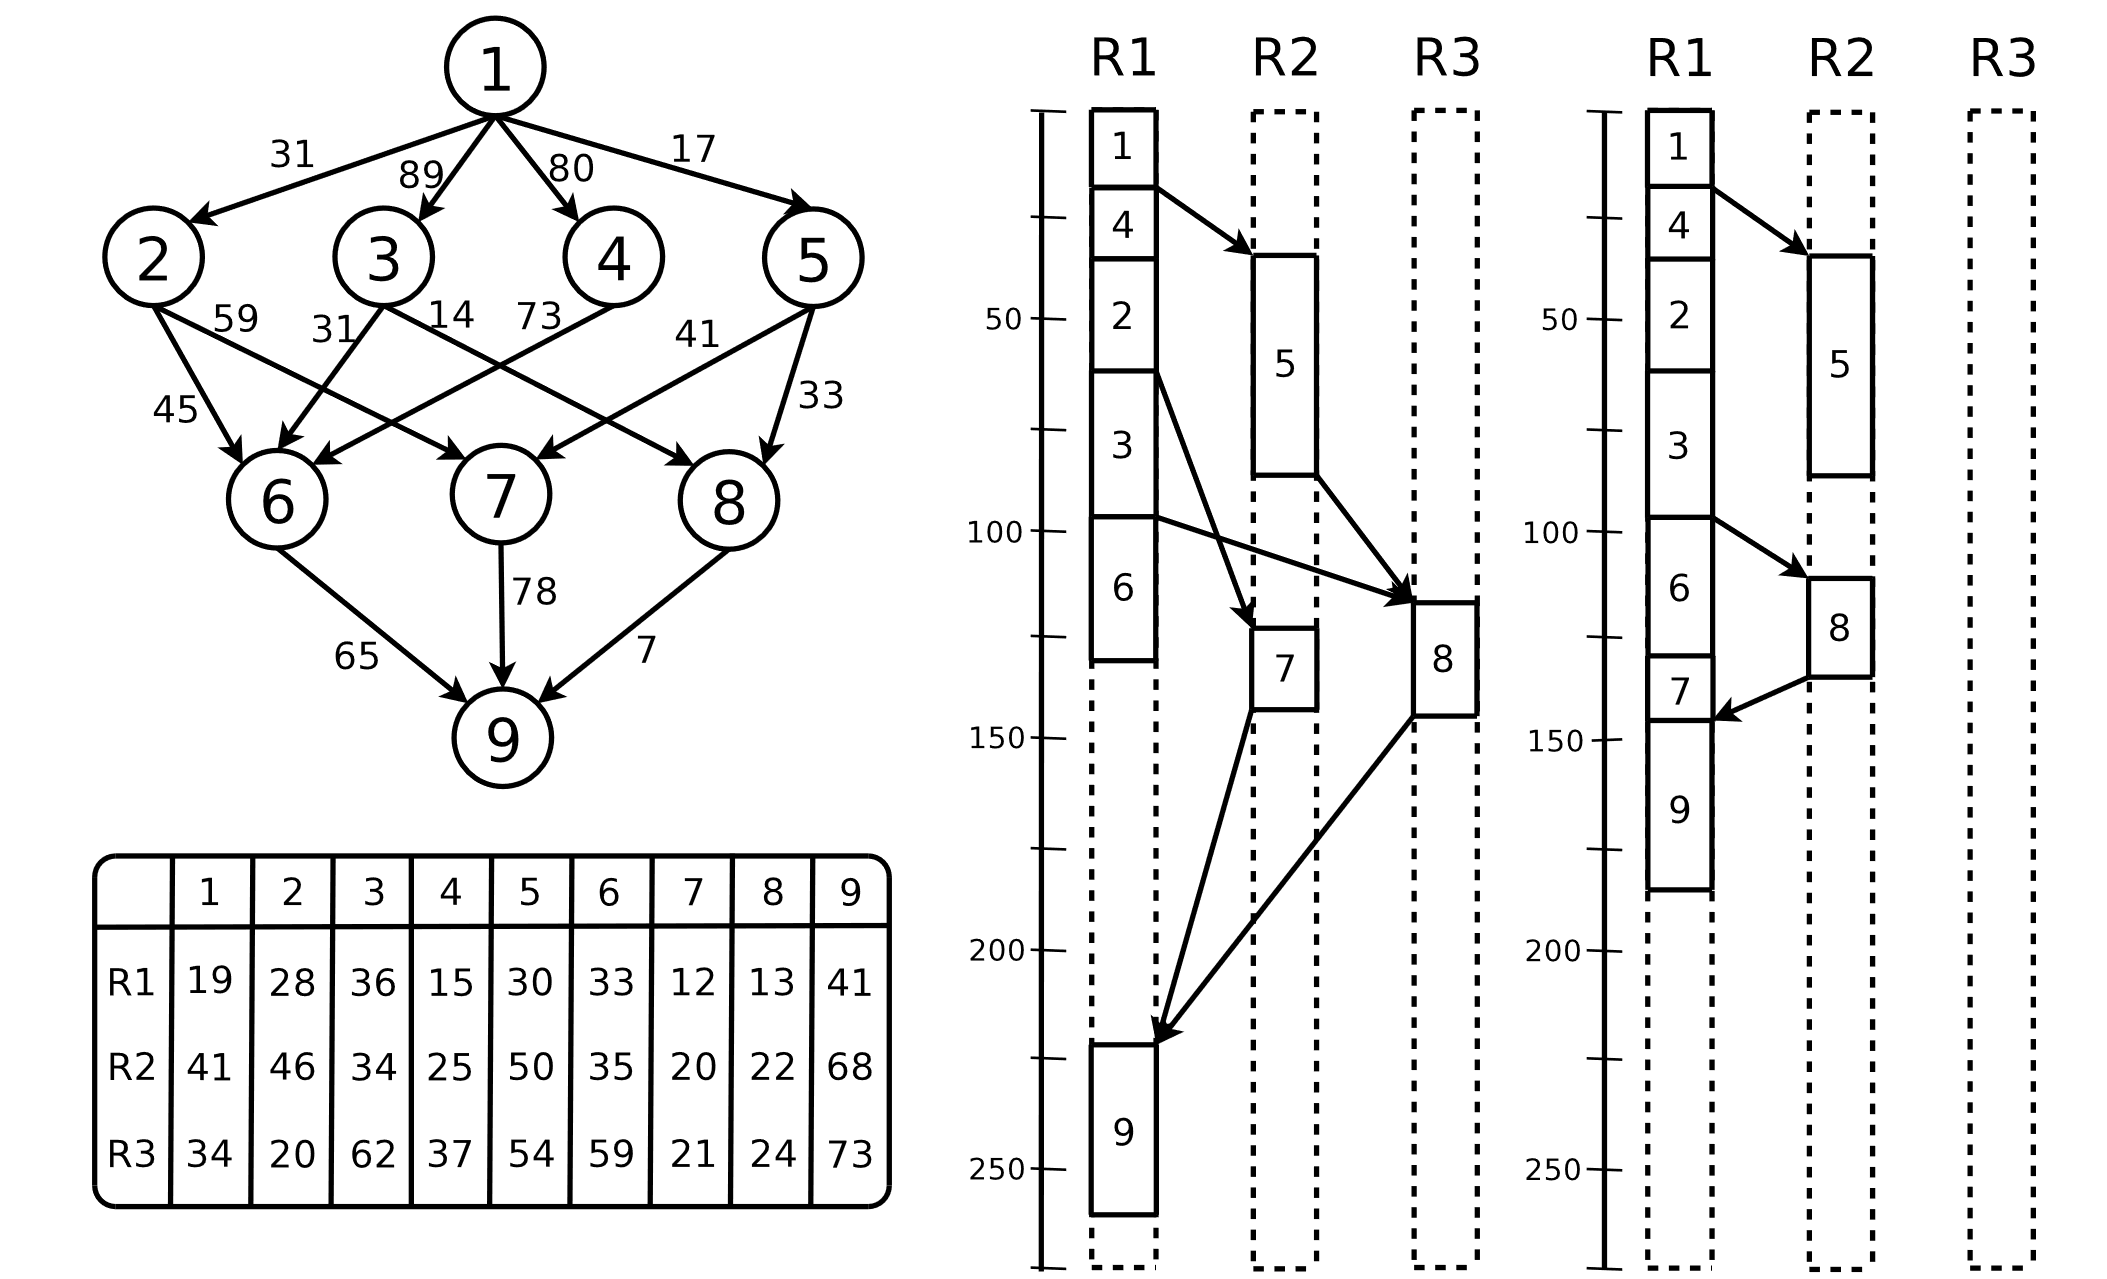
\includegraphics[width=0.85\textwidth]{heft_task_modeling}
        \bicaption{\quad 一种HEFT类算法\citep{topcuoglu_performance-effective_2002}对计算任务的建模}
        {\quad Modeling of heterogenous computing task by a HEFT like algorithm\citep{topcuoglu_performance-effective_2002}}
        \label{fig:heft_task_modeling}
    \end{figure}

    然而,因为该算法的贪心和短视特性,其性能在某些负载中离最优解相差很远,在之后的工作中,例如\citep{bittencourt_dag_2010},引入了有限的前瞻操作,使得在不增加太多时间复杂度的情况下让调度的最大完成时间相对于原算法平均约提升了20\%,之后的工作大多是为该算法添加其他的启发式步骤,如关键节点优先调度、悲观或乐观代价估计等等,但提升十分有限\citep{arabnejad_list_2014,zhou_list_2017}。
    
    HEFT类算法在最小的调度粒度是任务,这为该算法带来良好的可部署性的同时,也注定了在它的调度中不可能进行更细粒度的调度优化,从而最大限度地发挥硬件之间的并行性。因此总是存在着较多的空泡,甚至如图~\ref{fig:heft_task_modeling},会存在有些硬件从始至终都都维持着很低的利用率。且其算法偏向于将任务驻留在起始硬件节点上,对其他硬件利用率较低。

    \subsection{面向近存计算系统的调度技术研究与应用}
    
    由于架构和功耗的限制,PIM核心在局部性良好、计算密集型的负载运行时往往与CPU的性能存在着一定的差距,而CPU在运行局部性差、访存随机性高且不需要复杂运算的负载时,会面临很严重的访存瓶颈,此时PIM在总访存带宽上的优势会让其的性能远远强于CPU。然而,当任务调度不佳时,整个系统的能效比和性能会急剧下降,甚至出现负优化的现象\citep{gomez-luna_benchmarking_2021}。这也凸显了调度技术在近存计算系统实际应用上的重要性。也促生了一系列面向近存计算系统的调度技术研究。在相关调度技术研究中,不乏更细粒度的调度方法,此类研究通常会与近存计算系统自身特殊的体系结构设计紧密结合,同时涉及到对CPU硬件结构的修改,以完成更细粒度的调度优化,并期望利用硬件设计优化负载的调度和执行效率。
    
    在现有的工作中,针对近存计算系统,负载调度的思路大致分为两种:
    
    1. 从一致性入手:在尽可能少做数据搬移、保留近存计算带来的优势的情况下,通过在执行负载时维持数据块的一致性,从而做到CPU-PIM协同计算。一个典型的例子就是\citep{boroumand_lazypim_2017}中提出的惰性同步策略,该策略默认不使用同步,将不同任务地指令同时派发给CPU和PIM系统,使CPU和PIM乐观地共同执行涉及同一块存储的负载,并对TLB、页表结构和一致性协议进行定制,加入新的原子命令以处理完成工作的原子提交以及涉及脏数据块操作的原子回退机制,从而减少了内存总线中的通信总量。
    
    2. 从指令集扩展入手:通过扩展硬件,从而做到自动将访存密集型负载中的特定指令派发到至PIM系统中。一个典型的例子是工作\citep{ahn_pim-enabled_2015}里,在模拟器中对CPU硬件结构作出修改后,加入了局部性检测元件,并同时在CPU和PIM核心里扩展了新的、用于近存计算系统的特殊指令集。当运行时检测到局部性符合设定条件之后,CPU中特殊的控制器则会将特定指令派发到PIM元件上,以完成特定操作。通过这种依条件派发指令方式完成了CPU-PIM的协同计算。
    
    以上基于近存计算系统的负载调度策略,相对于~\ref{subsec:hetero_scheduling_intro}所描述的现实系统中的异构负载调度算法而言,其调度的单元从任务级细化到了指令级,可以在不改变编程模式的前提下完成更细粒度的CPU-PIM并行,但都涉及到对CPU和PIM内存本身硬件的修改,所以截至目前所有相关工作都是在模拟器中进行的,但是它们对该问题的解决思路,对基于实际DIMM近存计算系统负载调度框架的设计来说,仍具有很高的参考价值。

%%%%%%%%%%%%%%%%%%%%%%%%%%%%%%%%%%%%%%%%%%%%%%%%%%%%%%%%%%%%%%%%%%%%%%
\section{关键问题与研究目标}\label{sec:problems_and_goals}
    \subsection{存在的问题}\label{subsec:existed_problems}
    %访存密集型负载在真实计算任务中会与计算密集型交叉出现,任务判别问题
    %现实PIM系统与之前研究的模型不一致,实际应用时无法套用之前研究的成果去修改硬件
    %HEFT类算法粒度太粗,偏向于不去使用PIM系统
    %由于前几条,在现实PIM系统中,发挥其特殊架构优势时对调度的要求会额外的高
    本课题选用目前工具链与开发流程较为成熟的UPMEM商用近存计算系统作为实验平台,对该平台上负载的调度问题进行研究,由于其在近存计算领域被广泛使用并研究,具有一定的代表性,沿用~\ref{subsec:evolution_of_PNM}中的命名习惯,下文所述的“PIM计算系统”即专指“UPMEM商用近存计算系统”。
    
    在应用实际PIM计算系统时,尽管其特殊的体系结构在运行某些负载时提供了一系列引人注目的优势,其仍有若干关键问题亟待解决:
   
    首先,在负载方面,许多重要的计算负载都是访存密集与计算密集型任务混合的\citep{boroumand_lazypim_2017},此时只能依靠PIM和CPU进行协同才能获得最佳性能,然而对任务进行划分的方法、划分的粒度均是尚未被完美解决的问题。对于任务的分配以及CPU-PIM间通信策略的设计,会极大程度上影响整个系统的性能,甚至在许多情况下,依靠朴素地进行手动负载分配会导致显著的性能恶化,甚至是负优化(如图~\ref{fig:prim_benchmarks}中的NW、BFS等)。
    
    \begin{figure}[!htbp]
        \centering
        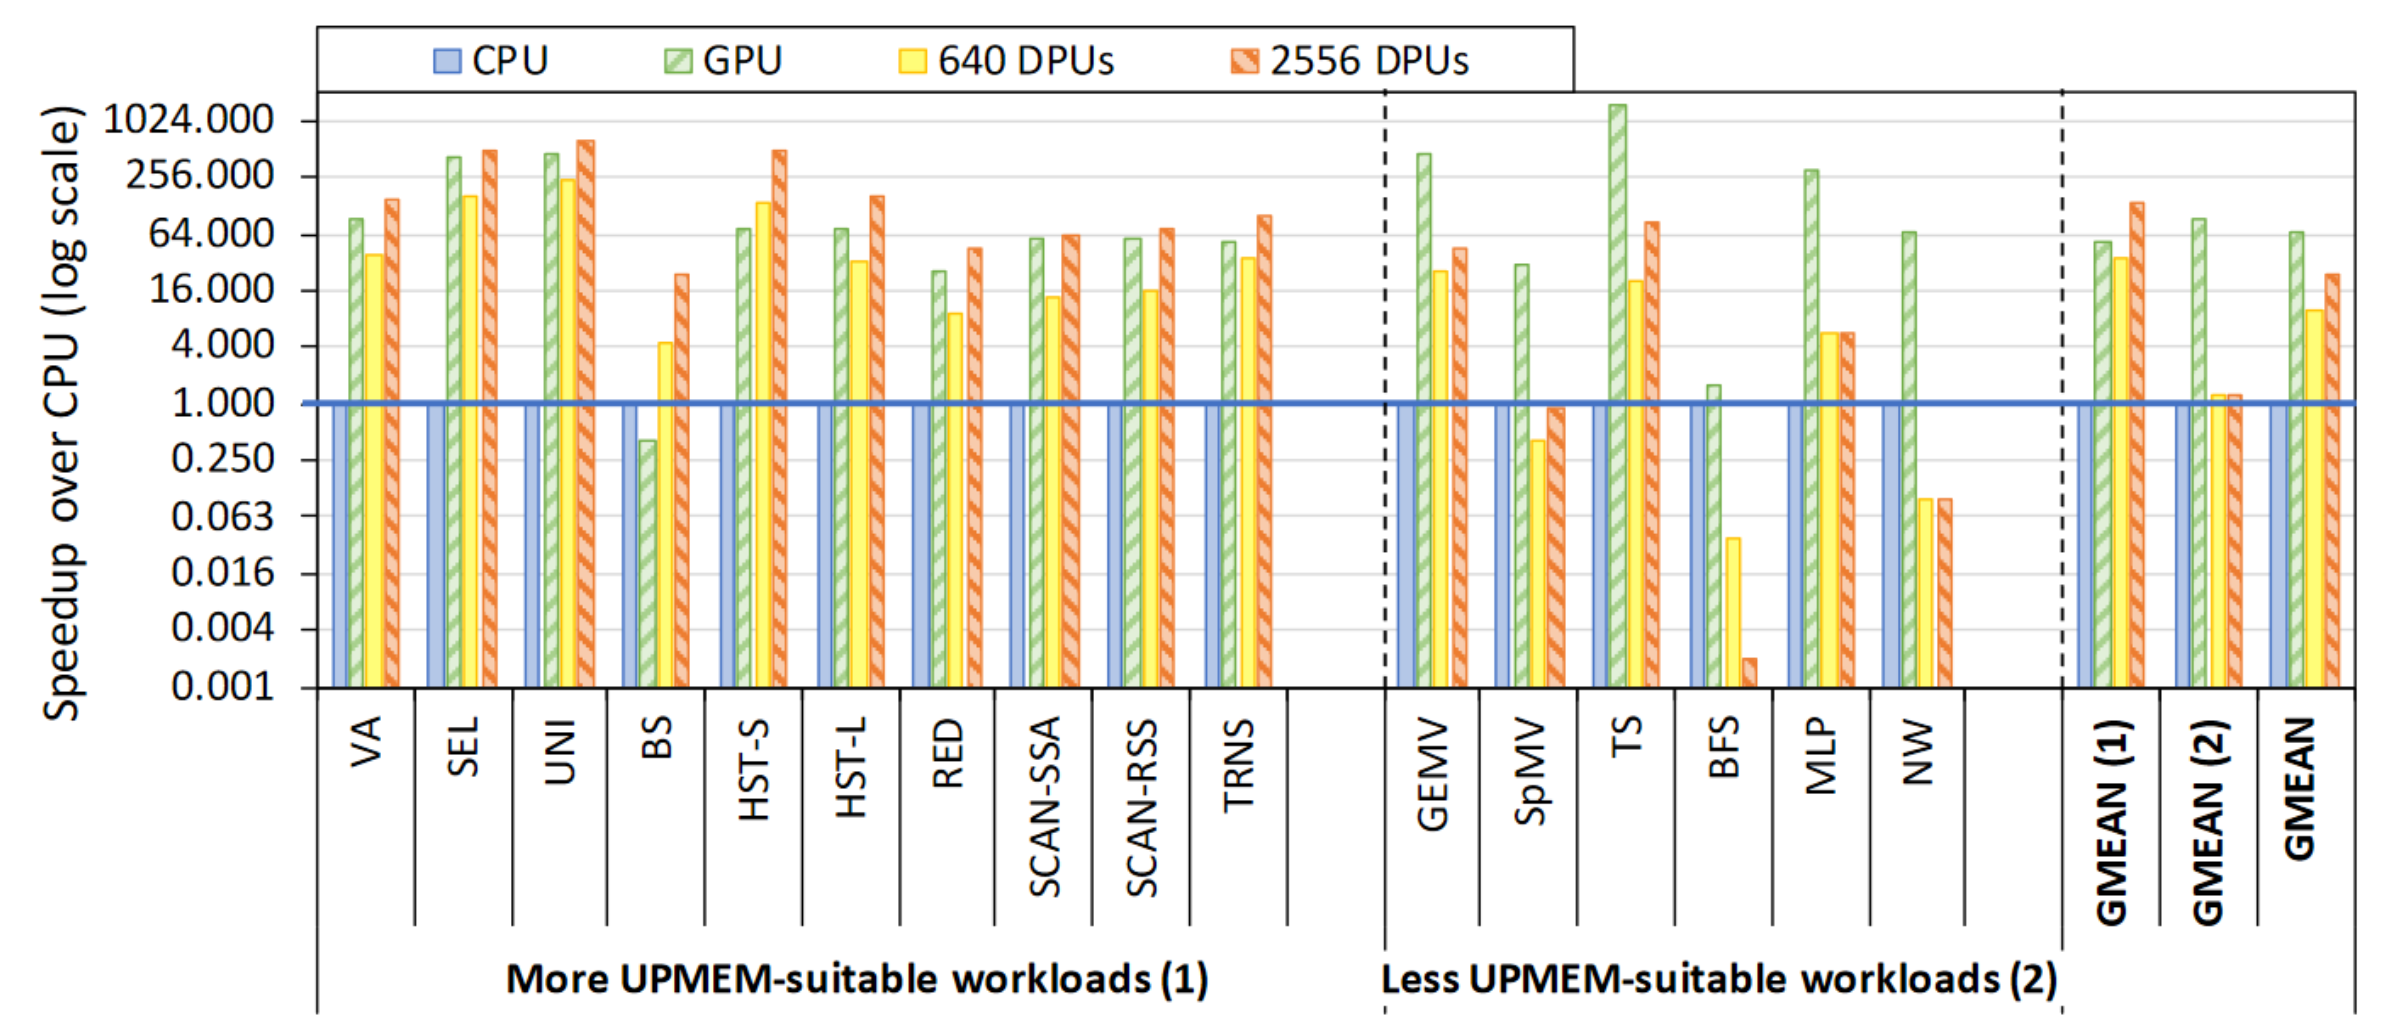
\includegraphics[width=0.85\textwidth]{prim-benchmarks}
        \bicaption{\quad 对基于DIMM的现实近存计算系统UPMEM的性能测试\citep{gomez-luna_benchmarking_2021}}
        {\quad Benchmarks of a real-world DIMM based PNM system, UPMEM\citep{gomez-luna_benchmarking_2021}}
        \label{fig:prim_benchmarks}
    \end{figure}
    
    其次,在硬件模型上,现实PIM计算系统的硬件结构与学术研究上所用的近存计算模型存在出入。本研究中所基于的PIM计算系统存在着若干个特征,显著区别于~\ref{subsec:evolution_of_PNM}中其他工作所基于的计算系统模型:
    
    \begin{enumerate}
        \item DRAM与PIM-MRAM非统一编址: UPMEM DIMM在使用中不与其他普通DIMM构成的主存储器统一编址寻址,获取其存储中的数据需要涉及到UPMEM-DIMM和主存储间的通信。
        \item PIM核间通信昂贵:UPMEM PIM核与核间不存在高速共享缓存和专用互联模块,所有PIM核间的通讯需要通过主存储器并由CPU直接介入,这会占用CPU资源以及访存带宽,带来很高的通信开销。
        \item 单个PIM-DPU只能直接进行小区间的PIM操作:单个UPMEM-DPU能通过DMA直接访问的空间只有64MiB,且区别于普通DIMM,UPMEM-DIMM在映射内存地址时不会将相邻的字节映射到不同颗粒上,而是会将8个相邻字节映射到同一个颗粒上的同一个DPU访存空间上。
        \item 近存计算内存不支持同时进行运算-传输:由于SDK底层将计算和传输抽象成同一类任务,并采用了任务队列的形式实现执行逻辑,UPMEM-DIMM无法在运行近存计算负载时处理与主存储器间的传输,以完成数据的预取和及时写回。
    \end{enumerate}

    此外,关于现有调度策略,目前主流的调度策略分为两种:或是基于贪心算法,依赖算法所调度的执行序,异步执行任务来完成任务间并行。又或是基于对CPU硬件结构本身的修改,依赖一致性协议或指令集扩展完成指令级并行,它们各自在优化任务分配、降低内存通信上取得了一定的成果,但是目前的方法在应用上的可行性和性能上仍次存在如下问题:
    \begin{enumerate}
        \item HEFT类算法无法使多器件协同处理一个任务,存在较多空泡;
        \item HEFT由于贪心策略,会导致短视,面对很高的通信代价,会偏向于自始至终将负载驻留在起始计算节点上。
        \item 基于一致性的调度策略对CPU做出结构性的修改,在现实系统中无法直接做到,且对于数据争用较为严重的负载,惰性同步会带来大量的回退开销。
        \item 基于指令集扩展的调度策略也对CPU结构进行了大量修改,且在复杂负载运行时,局部性判断器的决策质量会在很大程度上影响性能,造成较大开销。
    \end{enumerate}
    
    现有的工作或是因为执行逻辑不同、或是因为对硬件的改动,暂时无法直接应用于现实。
    
    最后,在执行逻辑上,以任务为粒度的调度框架所针对的负载模型和真实kernel的使用方式有着较大差异。而传统的函数级PIM kernel在使用时需要预先进行交叉编译,并在运行时传入UPMEM-DIMM中执行,这使得算子耦合性很强、灵活性较差,难以通过动态定制任务的执行逻辑和传输逻辑,以通过细粒度并行充分利用硬件资源。

    鉴于此,本工作将主要研究关于基于DIMM近存计算系统的调度技术,旨在结合现实近存计算系统,解决其在实际应用中存在的调度问题,从而更好地发挥近存计算体系结构在高性能计算领域的潜力。

    \subsection{研究目标}\label{subsec:research_goals}
    实际运行在近存计算系统的程序在处理任务卸载的过程中,一种朴素且被广泛使用的方法是依靠手动编程并管理管理负载的调度,将所有的负载分配和通信在程序编写时唯一确定。但这种“贪心式”的思路存在着弊端:当访存密集和计算密集型任务交替出现时,手动任务卸载中,过细粒度的同步或过粗粒度的任务划分,都会因频繁的数据搬移或过低的计算效率,从而带来不可忽视的性能开销,甚至会抵消近存计算带来的性能收益\citep{gomez-luna_benchmarking_2021,diab_high-throughput_2022}。一个可利用高层次任务信息进行调度,同时能结合硬件量化信息综合考虑到数据搬移开销、计算开销的调度策略是很有必要的。
    
    综合前文所述,当前近存计算系统存在着不同负载下性能差异大、运行负载时总体计算资源利用率低、CPU-PIM间数据搬移代价高等问题。且现有的异构调度算法在高代价数据搬移的前提下不能很好的利用计算资源,无法直接用于实际的近存计算系统的调度上。尽管现有的工作或是因为适用场景不同、或是因为对硬件的改动,暂时无法直接应用于现实。但它们仍存在着本文框架可以借鉴的思想:
    \begin{enumerate}
        \item 在任务内做到器件间的并行,应尽可能地消除异构器件闲等的情况,特别地,对于CPU-PIM这种双异构器件的系统,合适比例的负载划分所达成的器件间并行,会减少后续数据搬移所带来性能开销,从而起到预取作用。
        \item 基于贪心启发式算法对负载的调度会存在短视,从而形成局部最优解,在对于启发式的选择上,应尽可能采用更强的元启发算法以跳出局部最优。
        \item 基于局部性判断的调度方式,如PEI\citep{ahn_pim-enabled_2015},将局部性作为负载调度的唯一参考信息,但忽略了实际近存计算核心处理能力与CPU间的不匹配,且无法参考后续的任务信息以完成更大范围的调度,从根本上来说仍是短视且追求局部最优的。应利用高层次的任务信息从而尽可能避免短视决策所带来的性能损失。 
    \end{enumerate}
    
    为解决这些问题,本课题旨在基于实际的近存计算系统,研究并设计一种高性能、细粒度的调度方法,以实现对混合负载的细粒度任务划分和调度优化,从而得到相比于原有调度方法更高的性能与能效比。
    
    
    本课题的研究目标及设计可总结为以下三个要点:

    \textbf{混合负载类设计}
    
        目标:解决近存计算系统不同负载下性能差异大的问题。
        
        设计: 提出一种可细分、适用于CPU与PIM协同计算的异构负载类设计,通过算子层面的跨平台接口,实现任务分配与计算协同,为后续的模块设计建立基础。

    \textbf{基于混合负载类的协同计算框架设计}
    
        目标:提高运行负载时总体计算资源利用率。
        
        设计:基于混合负载类,设计调度策略生成模块。用先验知识进行任务分配的分治方法,包括量化器、回归拟合模块、策略价值判别模块及元启发策略优化器,以确定所有算子在不同器件上的任务分配比例,从而优化整体性能。

    \textbf{调度策略生成器与优化器设计}
        
        目标:降低负载间数据搬移代价,提高计算效率。
        
        设计:基于负载类的可分性,设计异步执行模块。利用细粒度异步并发执行缓解高传输代价带来的同步开销。并使用懒惰写回策略,最大限度地减少器件间传输空泡以及数据搬移开销,提高CPU-PIM系统整体的计算能力。
    
%%%%%%%%%%%%%%%%%%%%%%%%%%%%%%%%%%%%%%%%%%%%%%%%%%%%%%%%%%%%%%%%%%%%%%
\section{本文的贡献}\label{sec:contributions}
针对近存计算系统在实际应用时所面临的性能问题,本文提出了一系列创新性的解决方案。本文所涉及的贡献主要体现在以下几个方面:

\textbf{基于算子的负载抽象与跨平台算子基类的构建}

本文采用了一种以算子为核心的负载表达方式,并在此基础上设计并实现了一种新型的跨平台算子基类。这种基类不仅继承了算子表达方式的高内聚低耦合特性,便于编程实践和并行调度,而且通过重构UPMEM原有的工具链匹配了跨平台算子,增强了算子在不同计算环境中的适应性和可重用性。此外,该基类支持按比例调控不同计算单元的任务量,有效减少了因不当任务分配而引起的性能损耗,提升了负载执行的灵活性和效率。 通过这一综合性的贡献,本文在近存计算系统中实现了单一负载多设备执行的方法,还为异构计算环境中的算子设计与实现提供了一种新的范式,这对减少异构设备通信、提升计算任务的执行效率和系统的整体效能产生了积极影响。

\textbf{调度策略生成及优化模块}

本文基于混合负载类设计了一种新的调度策略生成及优化模块,用于生成并优化CPU-PIM间任务的调度。这种方法是一种基于先验知识的分治方法,能够有效提高计算资源的利用率。 具体到策略生成模块的构成,本文的贡献包括: 

	运行时性能量化器:本文开发了一个量化器,用于在预热阶段收集算子计算和传输的性能量化数据,为后续模块提供必要的性能数据。
 
	量化性能拟合模块:本文实现了一个回归拟合模块,用于建立和训练可泛化的性能模型,用于调度价值评估。 
 
	调度价值判别模块:本文设计了一个调度价值判别模块,可基于量化拟合数据用于评估调度策略的价值,并为优化器提供反馈。
 
        元启发调度优化器:本文复现并采用了若干元启发优化算法,用于在有限时间内搜索最优调度策略,以提高系统的性能与能耗比。
        
 总结来说,本文为现实基于DIMM近存计算系统执行混合负载时的性能优化提供了一种新型解决方案。通过以算子中心的负载表达、跨平台算子基类的设计以及基于元启发算法的调度优化器的设计,本文不仅解决了性能差异、数据搬移代价高和计算资源利用率低的问题,还提高了系统的计算性能与能效比,有望为推进基于DIMM的近存计算这一技术的实际应用做出一定贡献。
%%%%%%%%%%%%%%%%%%%%%%%%%%%%%%%%%%%%%%%%%%%%%%%%%%%%%%%%%%%%%%%%%%%%%%
\section{本文的组织}\label{sec:doc_organization}
第一章概述课题的研究背景与意义。
从存算单元性能发展所形成的“剪刀差”和存储墙现象入手,
介绍近存计算技术的研究背景,及其从设计理念到现实商业落地的发展历史,简要介绍了不同近存计算技术的设计思路和系统结构。
随后简要讲述了近存计算技术在应用时所面临的挑战,并阐述异构调度算法与本课题涉及研究内容的联系。
接着介绍了本文所涉及到的领域在国内外的研究现状,结合目前的主流方法引出研究中的
关键问题和研究目标。最后介绍了本文的贡献和组织结构。

第二章介绍了本课题所对应项目中涉及到的相关理论和技术。
首先,以粒度由粗到细的方式,依次介绍了目前主流的异构调度算法,以及面向PIM系统的细粒度调度方法。
随后介绍了本课题所设计的调度算法中所采用的的元启发优化算法。

第三章首先介绍了基于SKMD的负载执行时的基本流程。
随后结合UPMEM近存计算系统的负载执行流程以及常见性能瓶颈的归纳,
引出本课题对UPMEM-SKMD类型可分混合负载类的建模与设计,以及基于该负载建模的工具链重构。
随后介绍了该负载建模下的计算图执行逻辑的设计与实现,
同样以粒度从粗到细的顺序,依次介绍计算图执行逻辑中:算子间调度逻辑、算子间传输逻辑以及算子内计算逻辑的设计与实现,
并在最后对本章所设计并实现的基于SKMD的CPU-PIM协同计算框架进行总结

第四章主要介绍负载划分及调度优化算法的设计与实现。
由于本课题中的负载划分和调度优化会涉及到性能量化模型和元启发优化算法,
本章先从性能量化模型的训练流程和元启发参数优化的基本流程入手,
分别展开基于UPMEM的性能量化回归学习模块,以及面向负载量化回归学习模型的元启发调度优化模块的具体设计与实现
最后总结本章所介绍的负载划分及调度优化算法,
并对整个基于DIMM近存计算系统的调度优化方法进行系统讲解。

第五章主要介绍了本课题的实验结果和分析。
本章分为实验验证、验证结果和数据分析三段内容
首先介绍了测试数据集,分别介绍了测试中使用的不同计算特性的算子、不同拓扑结构的计算图
以及随机负载生成算法以及其最终生成的、用于本次测试的混合负载集合。
随后介绍了实验对结果的评价指标。
在验证结果部分,分别展示了算子性能量化回归模型的回归结果,不同负载中元启发调度优化算法的收敛情况,
以及经不同调度策略调度后,各个实验负载整体的性能和能耗情况。
在数据分析部分,分别对本课题所提出的调度算法进行优化效率、稳定性的分析,以及对调度结果进行进一步评估。

第六章则是对全文的总结,并提出未来可以继续研究与改进的方向。
